% !TEX program = xelatex
\documentclass[11pt]{article}
\usepackage{kotex}
\usepackage{booktabs}
\usepackage{siunitx}
\usepackage{pgfplots}
\usepackage{geometry}
\geometry{margin=1in}
\pgfplotsset{compat=1.18}
\sisetup{round-mode=places,round-precision=2}

% Set Korean fonts (kotex loads fontspec automatically)
\setmainhangulfont{NanumMyeongjo}
\setsanshangulfont{NanumGothic}
\setmonohangulfont{NanumGothic}

\title{RPL/BRPL 스트레스 실험 결과 보고서}
\author{}
\date{}

\begin{document}
\maketitle

\section*{개요}
본 문서는 RPL/BRPL 스트레스 테스트의 실행 환경, 실험 방법, 데이터 처리 절차,
그리고 측정 결과를 한국어로 정리한 LaTeX 보고서이다.
분석 데이터는 \texttt{results/summary.csv}와 \texttt{results/analysis/*.csv}를 기준으로 한다.

\section*{실험 환경}
\begin{itemize}
  \item 시뮬레이터: Cooja (Contiki-NG, headless 실행)
  \item 실행 방식: \texttt{cooja.jar -nogui <file.csc>} 형태의 CLI 실행
  \item 실행 스크립트: \texttt{run\_sweep\_stage1.sh}, \texttt{run\_sweep\_stage2.sh}, \texttt{run\_sweep\_stage3.sh}
  \item 로그 수집: \texttt{receiver\_root.c}의 CSV 출력 라인을 파싱
  \item 측정 시간: 총 360s (WARMUP=60s, MEASURE=300s)
  \item 재현성: seed 기반 실행
\end{itemize}

\section*{실험 설계}
\subsection*{공통 규칙}
\begin{itemize}
  \item 성능 지표는 MEASURE 구간에서만 계산
  \item 결과는 개별 실행 로그로부터 \texttt{summary.csv}로 집계
  \item 출력 구조:
  \begin{itemize}
    \item \texttt{results/raw/<stage>/<mode>/Nxx\_seedY\_srX\_irZ\_siT.\{csc,log,csv\}}
    \item \texttt{results/summary.csv}
    \item \texttt{results/thresholds.csv}
  \end{itemize}
\end{itemize}

\subsection*{Stage 1: N 스윕}
\begin{itemize}
  \item 고정: \texttt{SUCCESS\_RATIO=1.0}, \texttt{INTERFERENCE\_RATIO=1.0}, \texttt{SEND\_INTERVAL\_S=10}
  \item 노드 수: $\{5,10,15,20,25,30,40,50\}$
  \item Seed: $\{1,2,3\}$
  \item Mode: \texttt{rpl-classic}, \texttt{brpl}
\end{itemize}

\subsection*{Stage 2: 링크 품질 스윕}
Stage 1의 RPL classic 결과에서 N을 자동 선택:
\begin{itemize}
  \item Stable N: $PDR \ge 0.95$를 만족하는 가장 큰 N
  \item Marginal N: $0.90 \le PDR < 0.95$를 만족하는 가장 큰 N
  \item Marginal N이 없으면 stable N 위의 다음 N 사용
\end{itemize}

스윕 파라미터:
\begin{itemize}
  \item \texttt{SUCCESS\_RATIO} $\in \{1.0,0.95,0.9,0.85,0.8,0.75\}$
  \item \texttt{INTERFERENCE\_RATIO} $\in \{1.0,0.95,0.9,0.85\}$
  \item Seed: $\{1,2,3\}$
  \item Mode: \texttt{rpl-classic}, \texttt{brpl}
\end{itemize}

\subsection*{Stage 3: 트래픽 스윕}
Stage 2의 RPL classic 결과에서 knee 조건을 선택:
\begin{itemize}
  \item $0.85 \le PDR \le 0.92$인 조건이 있으면 0.90에 가장 가까운 조건 선택
  \item 없으면 0.90에 가장 가까운 조건 선택
\end{itemize}

스윕 파라미터:
\begin{itemize}
  \item \texttt{SEND\_INTERVAL\_S} $\in \{20,10,5,2\}$ (내림차순)
  \item Seed: $\{1,2,3\}$
  \item Mode: \texttt{rpl-classic}, \texttt{brpl}
\end{itemize}

\section*{지표 정의}
\begin{itemize}
  \item PDR: $ \mathrm{PDR} = \frac{\mathrm{rx\_count}}{\mathrm{tx\_expected}} $
  \item 평균 지연: $\mathrm{avg\_delay\_ms}$
  \item 95퍼센타일 지연: $\mathrm{p95\_delay\_ms}$
  \item 제어 오버헤드(초당): $ \mathrm{overhead\_per\_s} = \frac{\mathrm{dio\_count}+\mathrm{dao\_count}}{\mathrm{duration\_s}} $
\end{itemize}

\section*{붕괴 시점 탐지 기준}
\begin{itemize}
  \item 기본 기준: $\mathrm{PDR} < 0.9$ 또는 $\mathrm{rx\_count} \le 0$
  \item 스윕 순서: Stage 1은 N 증가, Stage 2는 success\_ratio 감소 후 interference\_ratio 감소,
  Stage 3은 send\_interval\_s 감소 순
\end{itemize}

\section*{분석 파이프라인}
\begin{itemize}
  \item 집계: \texttt{results/summary.csv}
  \item 붕괴 추정 및 비교 요약: \texttt{tools/r/analyze\_results.R}
  \item 결과 산출물: \texttt{results/analysis/collapse\_stage*.csv}, \texttt{mode\_stage\_comparison.csv}
\end{itemize}

\section*{모드/스테이지별 요약 통계}
\begin{table}[h]
\centering
\caption{모드/스테이지별 평균 요약}
\begin{tabular}{llrrrrr}
\toprule
Mode & Stage & PDR & Avg Delay(ms) & P95 Delay(ms) & Overhead/s & Runs \\
\midrule
brpl & stage1 & 0.00 & 0.00 & 0.00 & 2.67 & 69 \\
brpl & stage2 & 0.00 & 0.00 & 0.00 & 2.74 & 72 \\
brpl & stage3 & 0.00 & 0.00 & 0.00 & 3.15 & 12 \\
rpl-classic & stage1 & 1.00 & 382.21 & 574.57 & 10.59 & 121 \\
rpl-classic & stage2 & 1.00 & 456.99 & 943.87 & 24.38 & 173 \\
rpl-classic & stage3 & 1.00 & 418.27 & 690.10 & 24.03 & 12 \\
\bottomrule
\end{tabular}
\end{table}

\section*{붕괴 시점 요약}
\begin{table}[h]
\centering
\caption{Stage별 붕괴 조건(최초 발생 기준)}
\begin{tabular}{llrrrr}
\toprule
Mode & Stage & N & Success Ratio & Interference Ratio & Send Interval(s) \\
\midrule
brpl & stage1 & 5 & 1.00 & 1.00 & 10 \\
brpl & stage2 & 50 & 1.00 & 0.85--1.00 & 10 \\
brpl & stage3 & 50 & 1.00 & 1.00 & 2 \\
rpl-classic & stage1--3 & \multicolumn{4}{l}{붕괴 조건 미검출} \\
\bottomrule
\end{tabular}
\end{table}

\section*{Stage 2/3 상세 붕괴 조건}
\subsection*{Stage 2}
\begin{table}[h]
\centering
\caption{Stage 2 붕괴 조건 상세}
\begin{tabular}{lrrrrr}
\toprule
Mode & N & Success Ratio & Interference Ratio & PDR & Runs \\
\midrule
brpl & 50 & 1.00 & 0.85 & 0.00 & 3 \\
brpl & 50 & 1.00 & 0.90 & 0.00 & 3 \\
brpl & 50 & 1.00 & 0.95 & 0.00 & 3 \\
brpl & 50 & 1.00 & 1.00 & 0.00 & 3 \\
\bottomrule
\end{tabular}
\end{table}

\subsection*{Stage 3}
\begin{table}[h]
\centering
\caption{Stage 3 붕괴 조건 상세}
\begin{tabular}{lrrrrrr}
\toprule
Mode & N & Success Ratio & Interference Ratio & Send Interval(s) & PDR & Runs \\
\midrule
brpl & 50 & 1.00 & 1.00 & 2 & 0.00 & 3 \\
\bottomrule
\end{tabular}
\end{table}

\section*{시각화}
\subsection*{PDR 비교}
\begin{figure}[h]
\centering
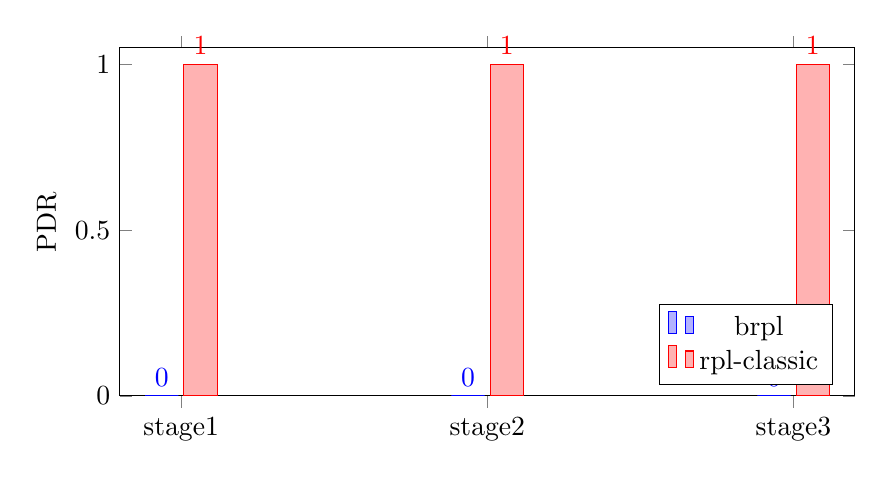
\begin{tikzpicture}
\begin{axis}[
  ybar,
  bar width=12pt,
  width=0.9\textwidth,
  height=6cm,
  ymin=0, ymax=1.05,
  ylabel={PDR},
  symbolic x coords={stage1,stage2,stage3},
  xtick=data,
  legend pos=south east,
  nodes near coords,
  nodes near coords align={vertical},
]
\addplot coordinates {(stage1,0.00) (stage2,0.00) (stage3,0.00)};
\addplot coordinates {(stage1,1.00) (stage2,1.00) (stage3,1.00)};
\legend{brpl,rpl-classic}
\end{axis}
\end{tikzpicture}
\caption{Stage별 평균 PDR 비교}
\end{figure}

\subsection*{제어 오버헤드 비교}
\begin{figure}[h]
\centering
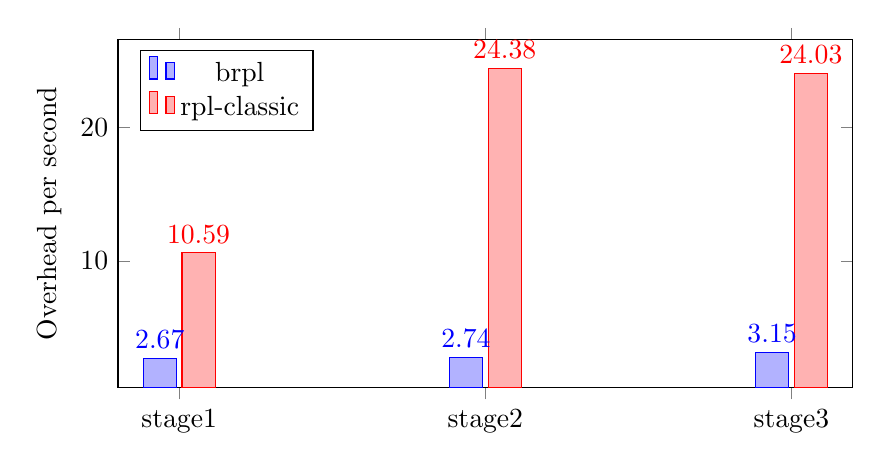
\begin{tikzpicture}
\begin{axis}[
  ybar,
  bar width=12pt,
  width=0.9\textwidth,
  height=6cm,
  ylabel={Overhead per second},
  symbolic x coords={stage1,stage2,stage3},
  xtick=data,
  legend pos=north west,
  nodes near coords,
  nodes near coords align={vertical},
]
\addplot coordinates {(stage1,2.67) (stage2,2.74) (stage3,3.15)};
\addplot coordinates {(stage1,10.59) (stage2,24.38) (stage3,24.03)};
\legend{brpl,rpl-classic}
\end{axis}
\end{tikzpicture}
\caption{Stage별 평균 제어 오버헤드 비교}
\end{figure}

\section*{해석 및 주의사항}
\begin{itemize}
  \item brpl은 모든 stage에서 PDR이 0으로 집계되어 초기부터 붕괴로 판정되었다.
  \item rpl-classic은 모든 stage에서 PDR이 1.0으로 유지되어 붕괴 조건이 관측되지 않았다.
  \item brpl 결과는 정상 송수신 여부, 로그 파싱, 프로토콜 설정을 추가 점검할 필요가 있다.
  \item \texttt{summary.csv}에는 동일 조건 중복 실행이 존재할 수 있으므로 결과 해석 시 주의한다.
\end{itemize}

\section*{재현 방법}
\begin{verbatim}
./run_sweep_stage1.sh
./run_sweep_stage2.sh
./run_sweep_stage3.sh
Rscript tools/r/analyze_results.R rpl-benchmark 0.9
\end{verbatim}

\end{document}
